% Created 2018-11-16 Fri 06:53
% Intended LaTeX compiler: pdflatex
\documentclass[uplatex, dvipdfmx]{jsarticle}
\usepackage[utf8]{inputenc}
\usepackage[T1]{fontenc}
\usepackage{graphicx}
\usepackage{grffile}
\usepackage{longtable}
\usepackage{wrapfig}
\usepackage{rotating}
\usepackage[normalem]{ulem}
\usepackage{amsmath}
\usepackage{textcomp}
\usepackage{amssymb}
\usepackage{capt-of}
\usepackage{hyperref}
\usepackage[utf8]{inputenc}
\usepackage[T1]{fontenc}
\usepackage{graphicx}
\usepackage{grffile}
\usepackage{longtable}
\usepackage{wrapfig}
\usepackage{rotating}
\usepackage[normalem]{ulem}
\usepackage{textcomp}
\usepackage{capt-of}
\usepackage{hyperref}
\usepackage{amsmath, amssymb}
\usepackage{pxjahyper}
\usepackage{listings}
\usepackage{fancyhdr}
\usepackage{mdframed}
\usepackage{here}
\usepackage{lscape}
\usepackage{physics}
\usepackage{okumacro}
\usepackage{framed}
\usepackage{xcolor}
\usepackage{multicol}
\usepackage{newtxtext}
\usepackage{newtxmath}
\usepackage{geometry}
\usepackage{mathtools}
\usepackage{subcaption}
\geometry{
top=2truecm, bottom=2truecm, left=1.5truecm, right=1.5truecm, includefoot}
\pagestyle{fancy}
\rhead{\thepage{}}
\mathtoolsset{showonlyrefs=true}
\author{B151235 山下直哉}
\date{2018/11/16}
\title{インテリジェントシステム 期末レポート}
\hypersetup{
  pdfauthor={B151235 山下直哉},
  pdftitle={インテリジェントシステム 期末レポート},
  pdfkeywords={},
  pdfsubject={},
  pdfcreator={Emacs 26.1 (Org mode 9.1.9)},
  pdflang={English},
  pdfborder={0 0 0},
  colorlinks=false,
  linkcolor=blue
}
\begin{document}

\maketitle

\section{Abstract}
\label{sec:org2bfde57}
授業において様々な手法での機械学習の理論を学習した。
このレポートは、理論学習の演習として将棋の駒の識別モデルを作成したことについて、結果と展望を記すものである。
識別器作成にはMicrosoft Azureが提供している、Custom Visionを使用した。
Custom Visionは千代田による「松屋警察」(2007)\footnote{ちょまどMadoka @chomado
\url{https://twitter.com/chomado/status/898812060624068609} - 2018/11/16 閲覧}(98\%の確率で松屋の牛丼を判定可能)など
有効なパフォーマンスを示した先行事例があり、手軽さも他のツールを圧倒している。
将棋の駒の判別として本来ならば、相手駒である反転駒を考慮して30クラス分類となるが、実際の対局のキャプチャ画像を使用したため
成銀の画像が入手できず、28クラス分類で識別器を作成した。
それぞれ100枚の画像を使用し、Precision:92.7\%, Recall:90.0\%の精度で識別ができる識別器を作成できた。
また、使用した全ツールはgithub\footnote{Detect Shogi-peacies by deep-leaning AI - conao3/shogi-detect
\url{https://github.com/conao3/shogi-detect} - 2018/11/16 閲覧}にて公開した。

\begin{multicols*}{2}
\section{先行事例研究}
\label{sec:org055d329}
インターネット上において機械学習分野ではすぎゃーんがTensor Flowによるアイドル顔識別器(2016)\footnote{TensorFlowによるアイドル顔識別器の話 - 2016.12.13 TensorFlow User Group \#2
\url{https://qiita.com/sugyan/items/f89cba95d67ab297d306} - 2018/11/16 閲覧}、その後改良を加え
2000人のアイドル顔を自力でタグ付けし1000人程度の識別が可能な識別器(2017)\footnote{TensorFlow と出会った「ドルヲタ」エンジニアが1年かけてたどり着いた境地 - LINE すぎゃーん(sugyan)氏
\url{https://press.forkwell.com/entry/2017/03/22/085525} - 2018/11/16 閲覧}などを作成し、機械学習の普及に寄与していた。

すぎゃーんのブログにおいて、将棋駒の分類を機械学習によって画像認識する話題\footnote{将棋駒画像の分類器をラクして作る
\url{https://memo.sugyan.com/entry/2018/05/02/182830} - 2018/11/16 閲覧}があり、Tensor Flowの
学習済みモデルを適用し識別器を作成していた。
そこでは識別の精度は悪く、研究は失敗したかのように書かれていた。
しかし、学習画像と検定画像は大きく異なっており(図\ref{fig:org1bd21dc})、
これをもって機械学習による画像識別機が将棋駒の判別に向いていないと帰結させるのは早計に思えた。

そこで私はNHK杯の録画から盤面が映されているコマを画像として保存し、その画像に対して学習し、
NHK杯の画像に対して識別することでどれだけの精度を持つ識別機が作成できるか研究した。

\begin{center}
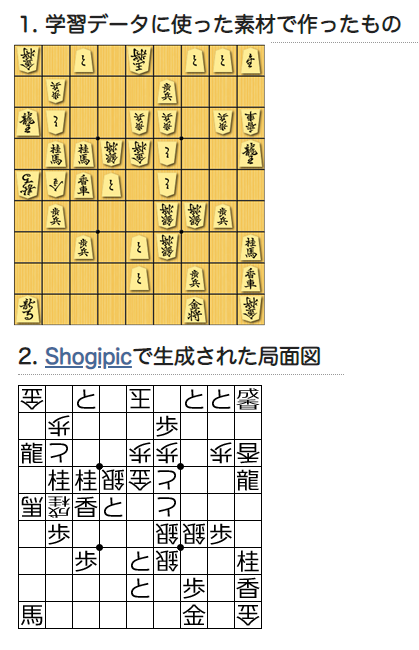
\includegraphics[width=6cm]{./sugyan.png}
\captionof{figure}{\label{fig:org1bd21dc}
すぎゃーんが使用した学習画像と検定画像}
\end{center}
\section{データ作成}
\label{sec:org545c546}
学習・検定データは以下の通り収集した。
\begin{enumerate}
\item NHK杯の映像を入手し、将棋盤の全面が写ったコマを手動で保存した。(盤面画像: 約200枚)
\item Pythonによる古典的な特徴解析により将棋盤領域を検出し、将棋盤領域のみの画像を作成した(図\ref{fig:orge62d96e})。
\item Pythonにより将棋盤領域のみの画像を \(9 \times 9\) のマス目画像にスライスした。(マス目画像: 約16,000枚)
\item PHPによるWebアプリケーションを作成し、手動で駒画像と空き画像に分類した(駒画像: 約5,000枚, 空白画像: 10,000枚: 33px \texttimes{} 33px)
\item 前段のアプリケーションにより、手動で28クラス分類を行った(図\ref{fig:org3aa5d60})。
\item サンプル数の足りない駒画像についてはPythonによりランダムノイズを与え、学習データを増やした。
\end{enumerate}

\begin{center}
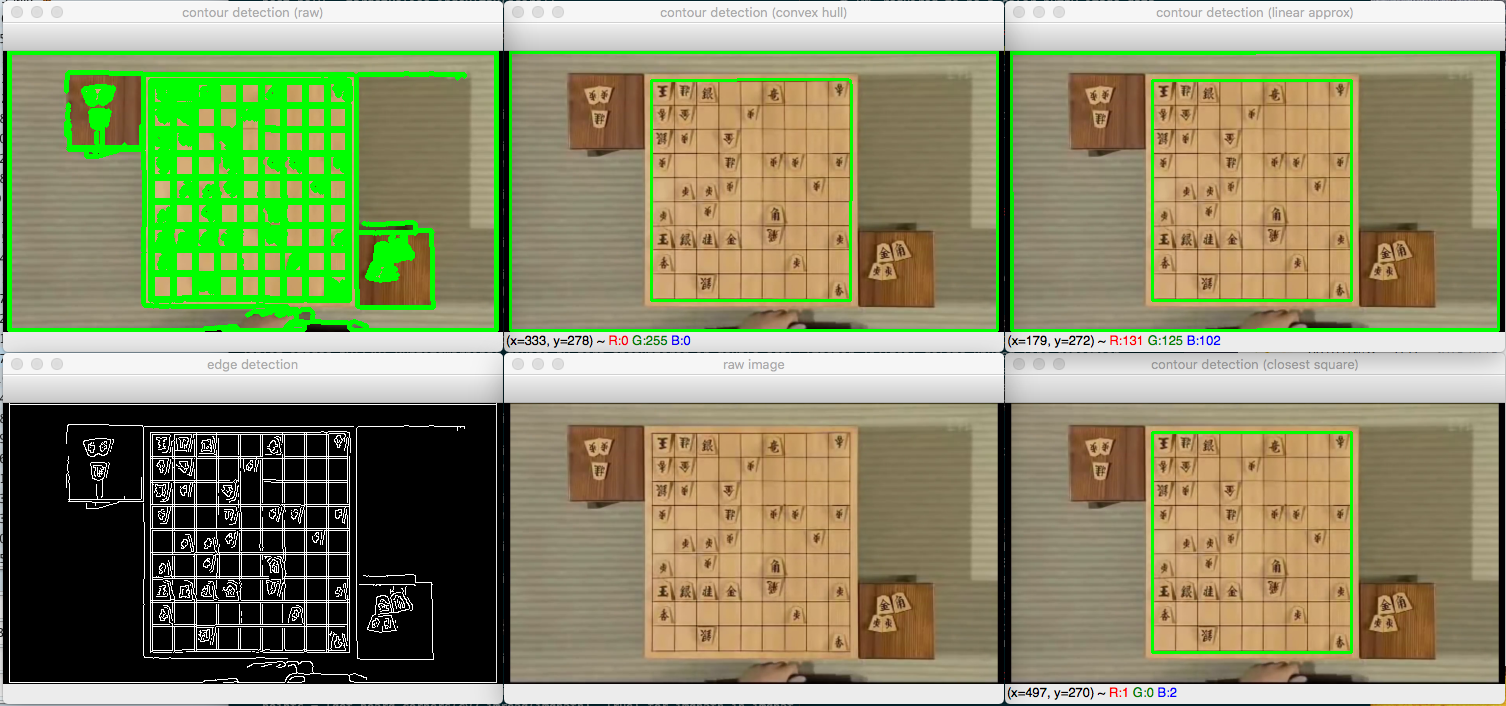
\includegraphics[width=9cm]{./python1.png}
\captionof{figure}{\label{fig:orge62d96e}
Pythonによる古典的な特徴解析}
\end{center}

\begin{center}
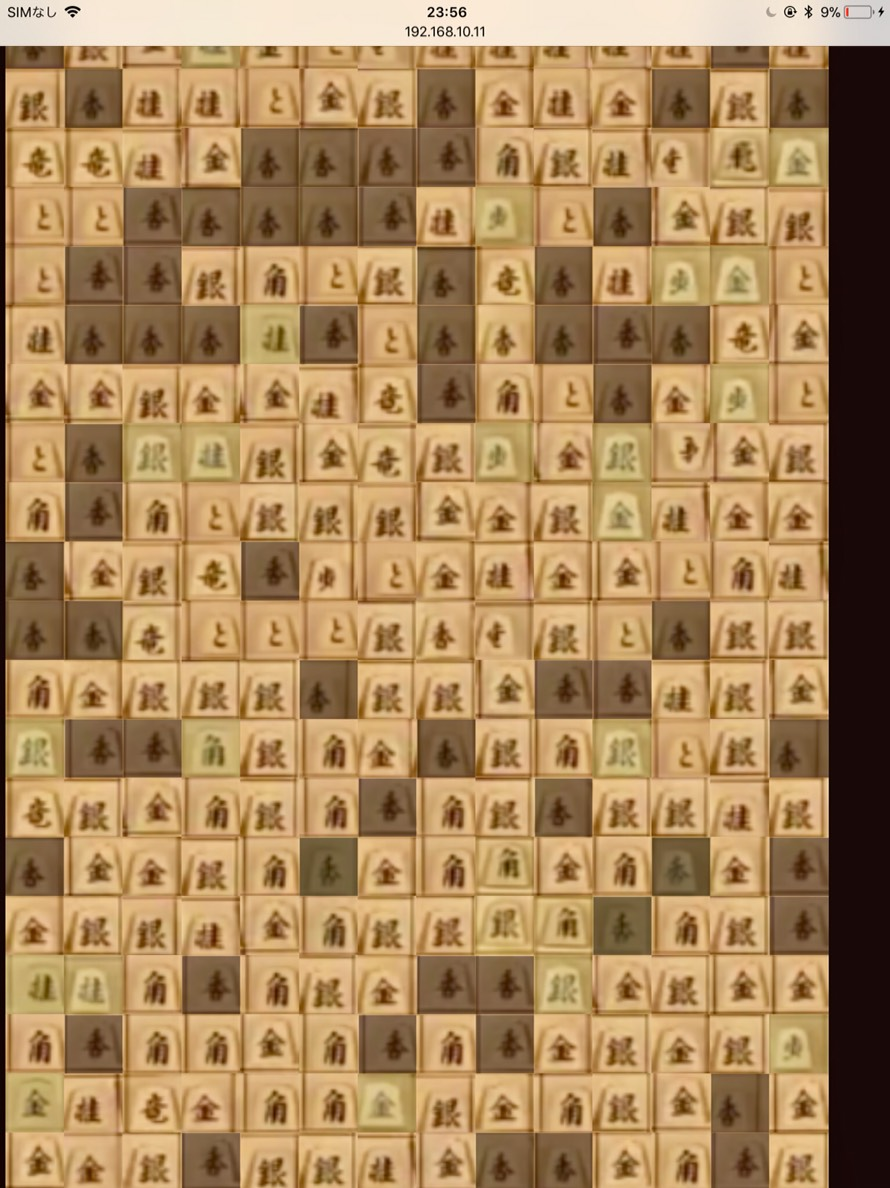
\includegraphics[width=5.5cm]{./php1.jpg}
\captionof{figure}{\label{fig:org3aa5d60}
PHPによるWebアプリケーションでの画像分類}
\end{center}
\section{学習・性能分析}
\label{sec:org02f7198}
本研究では識別器作成機としてMicrosoft AzureのCustom Vision\footnote{Microsoft Azure - Custom Vision
\url{https://www.customvision.ai} - 2018/11/16 閲覧}を選定した。
Custom Visionは1クラスにつき最低5枚、推奨50枚の画像を必要とし、画像をアップロード・タグ付けし、
「Train」ボタンを押すだけで識別器を作成できる。

Pythonによるランダムノイズを加え、各クラス3000枚の画像を用意したが、そのうち100枚の画像をアップロードし学習を行った。

結果としてPrecision: 92.7%, Recall: 90.0\%の識別器を作成できた(図\ref{fig:org726d3cd})。
クラス別に正答率を見ていくと、「桂馬」や「歩」の識別率が高く、「香車」や「成桂」の識別率が低かった。

\begin{center}
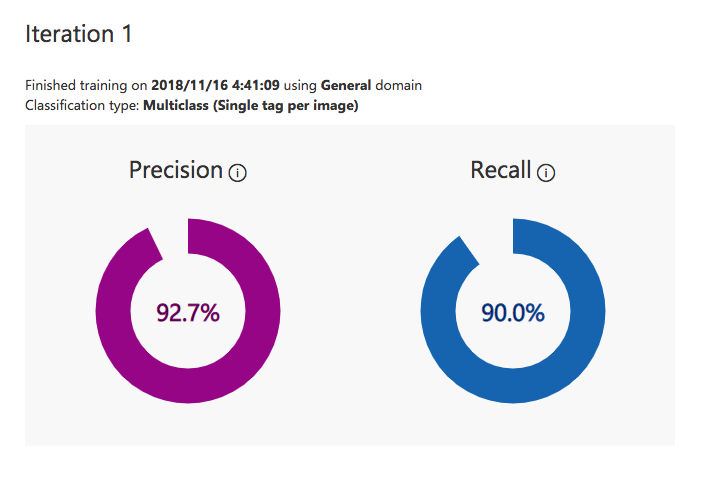
\includegraphics[width=4.5cm]{./azure1.png}
\captionof{figure}{\label{fig:org726d3cd}
Custom Visionによる識別器作成, 評価}
\end{center}
\section{考察}
\label{sec:org35035a5}
実際の対局映像のキャプチャを利用しているため、クラスにおいては極端に元データの少ないクラスが現れていた。
例えば識別率の低い結果となった「香車(Recall: 77.2\%)」については「歩」との混同が多い結果となった。
これは手動で分類する際にも目を細めて分類した難しい問題であり、もっと解像度の高い画像で行った場合、識別率が上がる可能性がある。
本研究においては1マスは33px正方形として正規化し扱ったため、100px正方形などでもう一度試してみたい。

また「成桂(Recall: 77.8\%)」については、本研究において、NHK杯の実際の対局から画像を入手したため「成桂」の元データを収集することが困難で、
200枚の盤面データから収集できた「成桂」元データはわずか10枚だった。
そのため学習データの大部分をPythonのランダムノイズにより生成された画像であり、それに由来し正答率が低くなってしまったと考えられる。

今後はTensor Flowなどを利用してDeep learningを利用した識別器を作成したい。
\end{multicols*}
\end{document}
